\documentclass[12pt]{beamer}

% Use metropolis theme. Show the progress bar but don't number slides
\usetheme[progressbar=frametitle, numbering=none]{metropolis}

% Set font with FiraSans, using lining figures everywhere
\usepackage[lf]{FiraSans}

% Use small caps in the titles of frames
\metroset{titleformat=smallcaps}

% Use metropolis' mLightBrown to emphasize
\renewcommand{\emph}[1]{{\color{mLightBrown}#1}}

% Set alert text in metropolis' mLightGreen
\setbeamercolor{alerted text}{fg=mLightGreen}

\usepackage{bm}
\usepackage{hyperref}
\usepackage{graphicx}
\graphicspath{{fig/}}

% Margins
\setbeamersize{text margin left=0.95cm, text margin right=0.95cm}

% Add slides after presentation (in case of questions), but don't include in progress bar
\usepackage{appendixnumberbeamer}

\title{Collective behaviour}
\subtitle{Parameter inference for model comparison}
\author{Jack Walton}
\date{June 19, 2019}
\institute{Newcastle University}

\begin{document}

\maketitle

\begin{frame}{What's it all about?}
  \centering
  \vspace{0.85cm}
  % Add more vertical space between rows
  \renewcommand{\arraystretch}{2.4}
  \begin{tabular}{@{}cc@{}}
    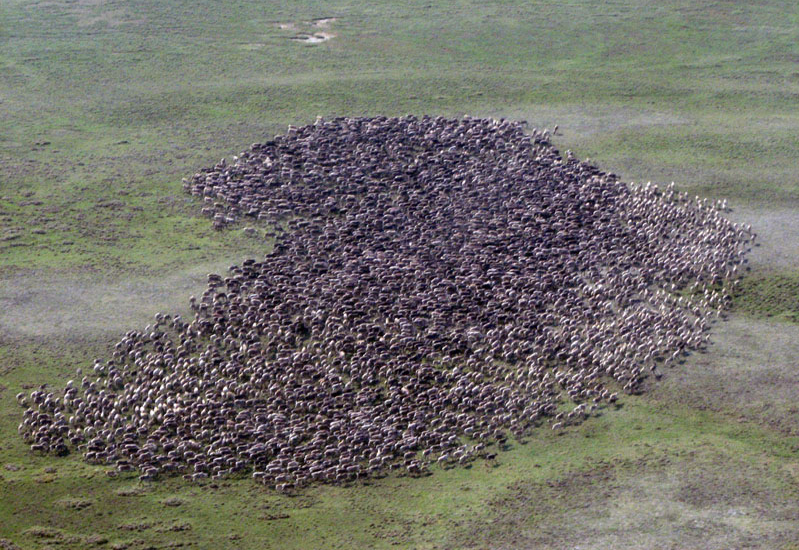
\includegraphics[width=0.4\textwidth]{caribou.jpg}              &
    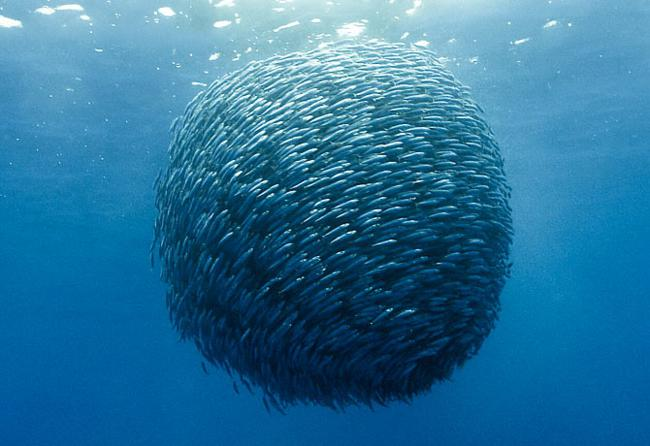
\includegraphics[width=0.4\textwidth]{milling_fish.jpg}           \\
    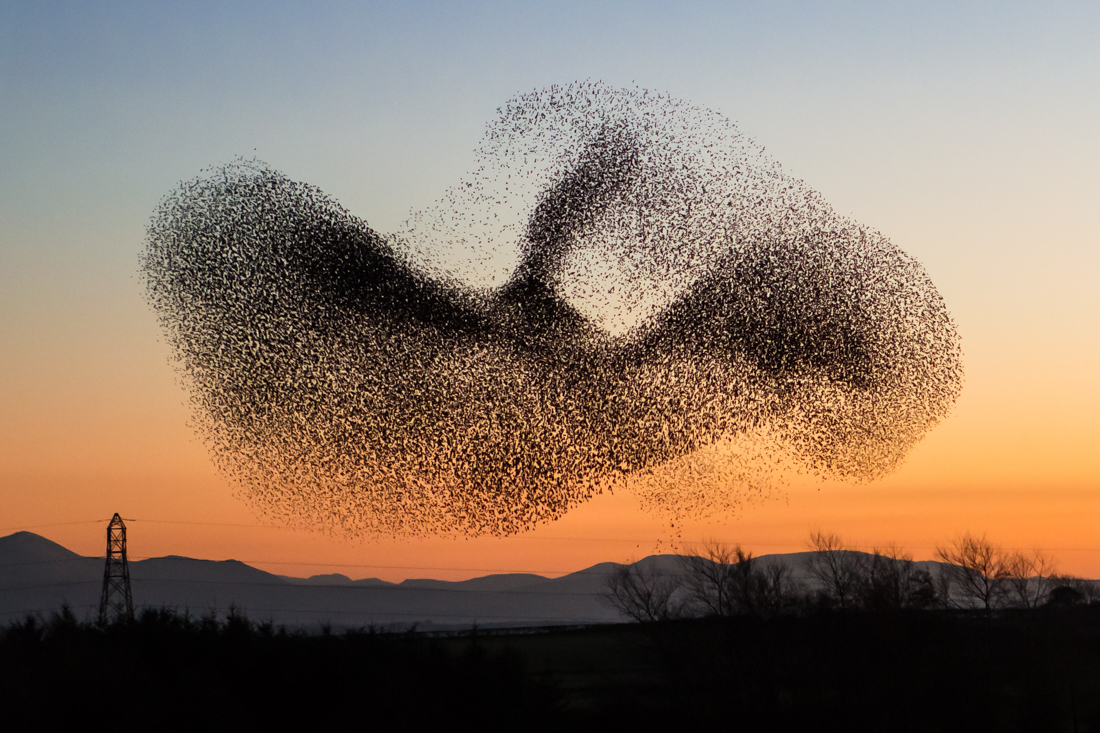
\includegraphics[width=0.4\textwidth]{starling_murmuration.jpg} &
    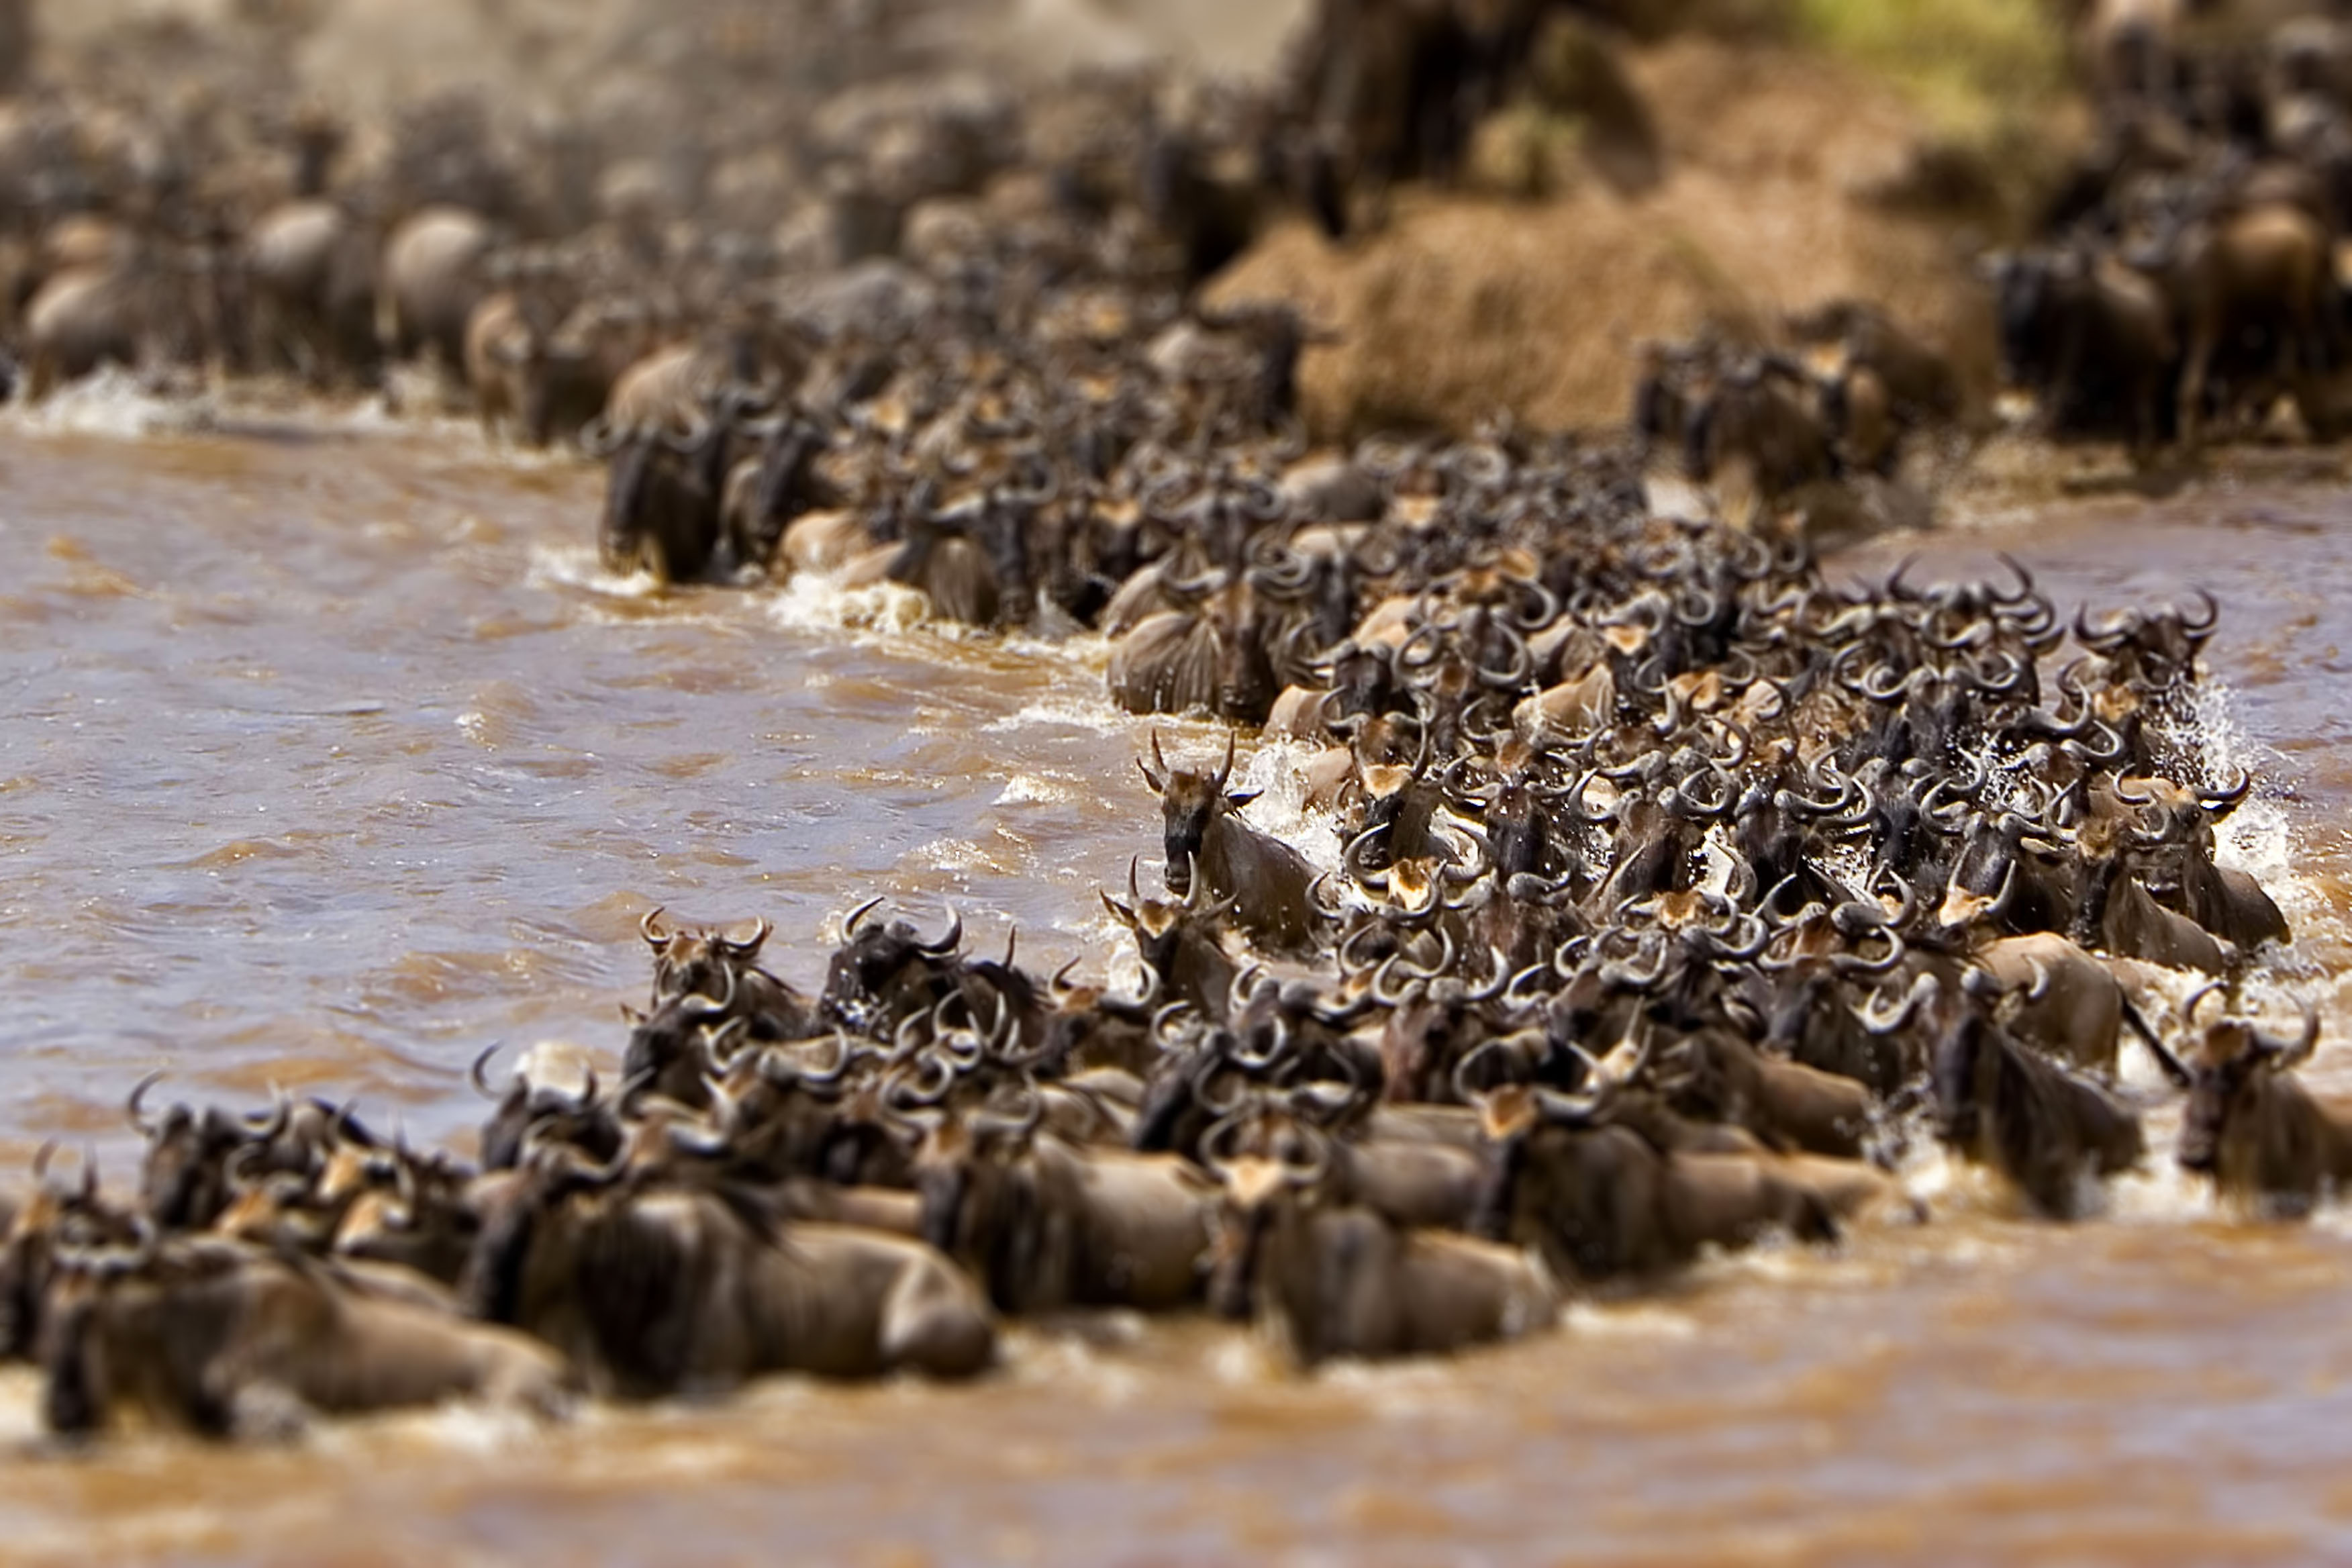
\includegraphics[width=0.4\textwidth]{wildebeest.jpg}
  \end{tabular}
\end{frame}

\begin{frame}{Where's the maths?}
  \begin{itemize}
    % Add more vertical space between items (should really do globally)
    \setlength\itemsep{1em}
    \item Many \emph{agent-based models} (ABMs) have been proposed to try explain collective
          motion
    \item ABMs follow a \emph{Lagrangian} approach, where behaviour is modelled at an individual
          level
    \item \alert{Simple rules} compound to create \alert{complex behaviour}
  \end{itemize}
\end{frame}

\begin{frame}{Where do we fit in?}
  \begin{itemize}
    \setlength\itemsep{1em}
    \item Loads of different ABMs have been proposed
    \item Very little \alert{quantitative} comparison between model and data
    \item Working in a \emph{Bayesian} paradigm we to seek carry out rigorous model verification /
          falsification
  \end{itemize}
\end{frame}

\begin{frame}{Our dataset}
  \begin{itemize}
    \setlength\itemsep{1em}
    \item Courtesy of Hayley Moore of the CDT programme
    \item Tracks positions of flocking sheep through time
          % Videos removed after talk
    \item \alert{\href{https://jwalton.info/assets/pgr_2019/vid1.mp4}{Raw data}}
    \item \alert{\href{https://jwalton.info/assets/pgr_2019/vid2.mp4}{Extracted data}}
  \end{itemize}
\end{frame}

\begin{frame}{The model}
  Positional update:
  \begin{equation*}
    \bm{x}_{i, t+1} = \bm{x}_{i, t} + \bm{v}_{i, t}
  \end{equation*}

  Directional update:
  \begin{equation*}
    \theta_{i, t+1} = \text{atan2}\,\Bigg({\sum_{j=1}^N \omega_{ij, t} \sin \theta_{j, t},
      \sum_{j=1}^N \omega_{ij, t} \cos \theta_{j, t}}\Bigg)
    + \epsilon_{i, t}
  \end{equation*}
  where $\epsilon_{i, t} \sim N(0, \alert{\sigma_{Y_i}})$ and
  \begin{equation*}
    \omega_{ij, t} = \frac{1}{\sqrt{2\pi\alert{\sigma_{X_i}}^2}}
    \exp{\bigg(\frac{-d_{ij, t}^2}{2\alert{\sigma_{X_i}}^2}\bigg)}
  \end{equation*}
\end{frame}

\begin{frame}{In summary}
  The model:
  \begin{itemize}
    \setlength\itemsep{1em}
    \item Each individual's behaviour is controlled by two parameters, \alert{$\sigma_{X_i}$}
          and \alert{$\sigma_{Y_i}$}
          \begin{itemize}
            \setlength\itemsep{0.3em}
            \item $\alert{\sigma_{X_i}}$ controls how \alert{strongly} agent $i$ \alert{interacts}
                  with neighbours
            \item $\alert{\sigma_{Y_i}}$ controls how much \alert{noise} agent $i$ \alert{experiences}
          \end{itemize}
  \end{itemize}

  Our goal:
  \begin{itemize}
    \setlength\itemsep{1em}
    \item Infer values of $\sigma_{X_i}$ and $\sigma_{Y_i}$ for every sheep in our dataset
  \end{itemize}
\end{frame}

\begin{frame}{A black box solution with STAN}
  \begin{itemize}
    \setlength\itemsep{1em}
    \item Stan is a probabilistic programming language, similar to BUGS and JAGS.
    \item Implements \emph{NUTS} algorithm --- a variant of \emph{HMC}
          \begin{itemize}
            \setlength\itemsep{0.3em}
            \item \alert{Input}: data and model specification
            \item \alert{Output}: posterior densities of parameters
          \end{itemize}
  \end{itemize}
\end{frame}

\begin{frame}{Results: posterior densities}
  \vspace{0.85cm}
  \centering
  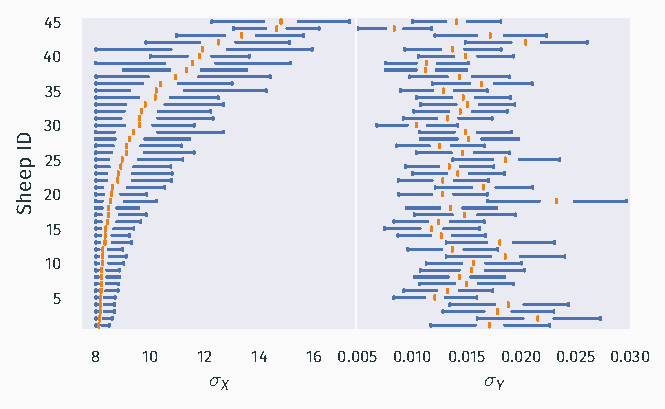
\includegraphics{summary_output.pdf}
\end{frame}

\begin{frame}{Results: forward simulations}
  \vspace{0.85cm}
  \centering
  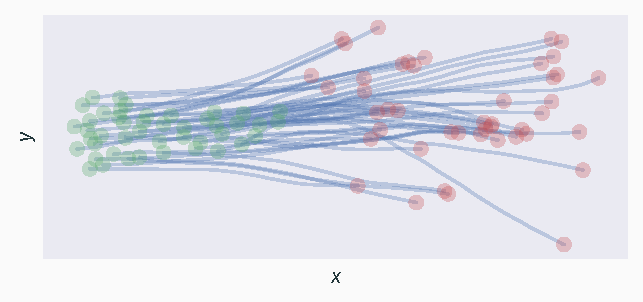
\includegraphics{forward_sim.pdf}
\end{frame}

\begin{frame}{Current model fitting}
  As an $AR(p)$ model:
  \begin{align*}
    \theta_{i, t+1} = \text{atan2}\,\Bigg(
     & \sum_{k=1}^p \sum_{j=1}^N \varphi_{j, t-k+1} \omega_{ij, t-k+1} \sin \theta_{j, t-k+1}, \\
     & \sum_{k=1}^p \sum_{j=1}^N \varphi_{j, t-k+1} \omega_{ij, t-k+1} \cos \theta_{j, t-k+1}
    \Bigg) + \epsilon_{i, t}
  \end{align*}

  As a topological model:
  \begin{align*}
    \theta_{i,t+1} = \text{atan2}\,\Bigg(
     & \sum_{j\in\mathcal{N}_{i,t}} \sin(\theta_{j,t})
    + n_i \text{ mod } \lfloor n_i\rfloor \sin(\theta_{j_*, t}), \\
     & \sum_{j\in\mathcal{N}_{i,t}} \cos(\theta_{j,t})
    + n_i \text{ mod } \lfloor n_i\rfloor \cos(\theta_{j_*, t}) \Bigg) + \epsilon_{i, t}
  \end{align*}
\end{frame}

\begin{frame}[standout]
  Questions?
\end{frame}

\appendix

% Try pre-empt questions
\begin{frame}
  \vspace{0.85cm}
  \centering
  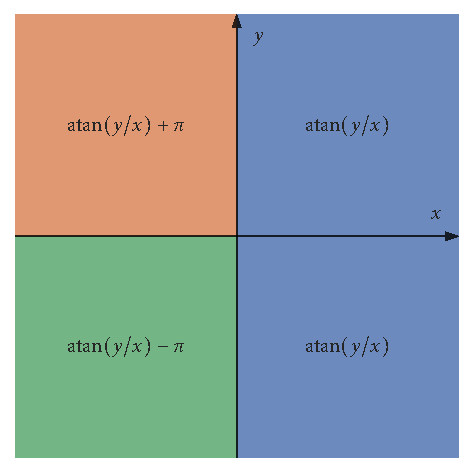
\includegraphics{atan_quadrants.pdf}
\end{frame}

\begin{frame}
  \vspace{0.85cm}
  \centering
  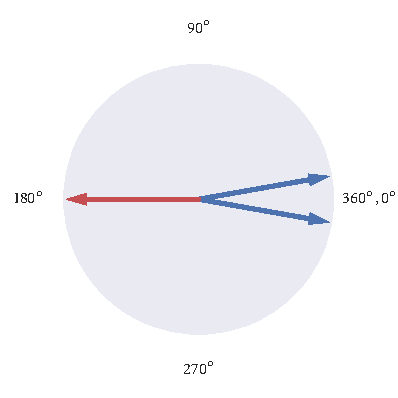
\includegraphics[width=0.5\textwidth]{arith_mean.pdf}%
  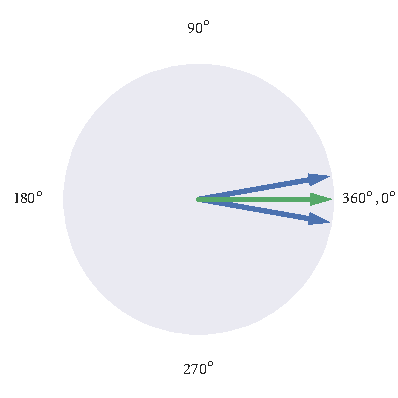
\includegraphics[width=0.5\textwidth]{circ_mean.pdf}
\end{frame}

\begin{frame}
  \vspace{0.85cm}
  \centering
  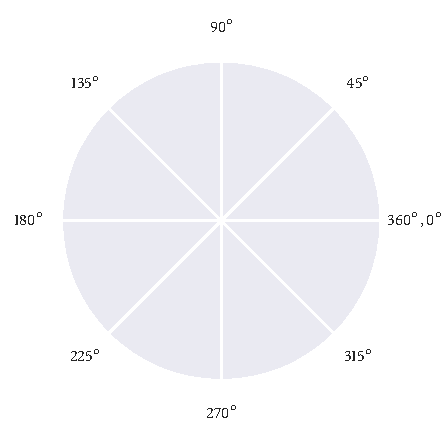
\includegraphics[width=0.5\textwidth]{degree_axes.pdf}%
  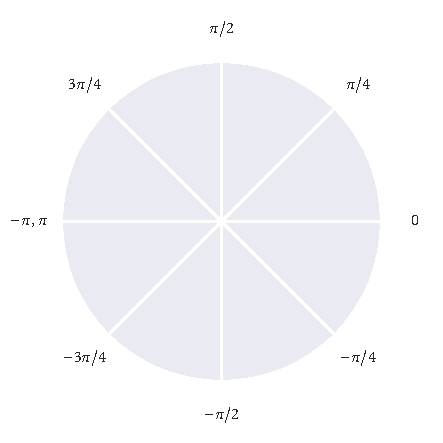
\includegraphics[width=0.5\textwidth]{radian_axes.pdf}
\end{frame}

\end{document}
